\documentclass{sigchi}

% Use this command to override the default ACM copyright statement (e.g. for preprints). 
% Consult the conference website for the camera-ready copyright statement.


%% EXAMPLE BEGIN -- HOW TO OVERRIDE THE DEFAULT COPYRIGHT STRIP -- (July 22, 2013 - Paul Baumann)
% \toappear{Permission to make digital or hard copies of all or part of this work for personal or classroom use is 	granted without fee provided that copies are not made or distributed for profit or commercial advantage and that copies bear this notice and the full citation on the first page. Copyrights for components of this work owned by others than ACM must be honored. Abstracting with credit is permitted. To copy otherwise, or republish, to post on servers or to redistribute to lists, requires prior specific permission and/or a fee. Request permissions from permissions@acm.org. \\
% {\emph{CHI'14}}, April 26--May 1, 2014, Toronto, Canada. \\
% Copyright \copyright~2014 ACM ISBN/14/04...\$15.00. \\
% DOI string from ACM form confirmation}
%% EXAMPLE END -- HOW TO OVERRIDE THE DEFAULT COPYRIGHT STRIP -- (July 22, 2013 - Paul Baumann)


% Arabic page numbers for submission. 
% Remove this line to eliminate page numbers for the camera ready copy
% \pagenumbering{arabic}


% Load basic packages
\usepackage{balance}  % to better equalize the last page
\usepackage{graphics} % for EPS, load graphicx instead
\usepackage{times}    % comment if you want LaTeX's default font
\usepackage{url}      % llt: nicely formatted URLs

% llt: Define a global style for URLs, rather that the default one
\makeatletter
\def\url@leostyle{%
  \@ifundefined{selectfont}{\def\UrlFont{\sf}}{\def\UrlFont{\small\bf\ttfamily}}}
\makeatother
\urlstyle{leo}


% To make various LaTeX processors do the right thing with page size.
\def\pprw{8.5in}
\def\pprh{11in}
\special{papersize=\pprw,\pprh}
\setlength{\paperwidth}{\pprw}
\setlength{\paperheight}{\pprh}
\setlength{\pdfpagewidth}{\pprw}
\setlength{\pdfpageheight}{\pprh}

% Make sure hyperref comes last of your loaded packages, 
% to give it a fighting chance of not being over-written, 
% since its job is to redefine many LaTeX commands.
\usepackage[pdftex]{hyperref}
\hypersetup{
pdftitle={Collaborative Multimodal Annotation System for Peer Discussion at Scale},
pdfauthor={LaTeX},
pdfkeywords={SIGCHI, proceedings, archival format},
bookmarksnumbered,
pdfstartview={FitH},
colorlinks,
citecolor=black,
filecolor=black,
linkcolor=black,
urlcolor=black,
breaklinks=true,
}

% create a shortcut to typeset table headings
\newcommand\tabhead[1]{\small\textbf{#1}}


% End of preamble. Here it comes the document.
\begin{document}

\title{Multimodal Peer Discussion at Scale}

\numberofauthors{3}
\author{
  \alignauthor Dongwook Yoon\\
    \affaddr{Cornell University}\\
    \affaddr{Ithaca, NY 14850}\\
    \email{dy252@cornell.edu}\\
  \alignauthor Piotr Mitros\\
    \affaddr{edX}\\
    \affaddr{Cambridge, MA 02139}\\
    \email{pmitros@edx.org}\\
}

\maketitle

\begin{abstract}
Abstract
\end{abstract}

\keywords{
	Massive open online courses; peer discussion; multimodal annotation; voice user interface; peer group assignment.
}

\category
{H.5.3.} Group and Organization Interfaces: Collaborative computing; {H.5.2.} User Interfaces: Interaction styles; {H.5.1.} Multimedia Information Systems: Audio input/output.

\section{Introduction}

Peer-discussion is an important interactive learning activity that can strengthen students’ mental model about classroom concepts \cite{nicol2003peer} and broaden their perspective on problem solving \cite{smith2009peer}.
Massive open online course providers endeavored to provide a large number of students with online peer discussion activities through discussion forums or video chats.
However, those communication tools does not support both of the rich face-to-face like communication modalities and the flexibility of asynchronous interaction together.

Recently, Yoon et al. presented a multimodal annotation system called RichReview \cite{yoon2014richreview}.
RichReview brought expressivity of multimedia recording into asynchronous document annotations.
Although the original system was built for the writing feedback purpose, we acknowledged the potential of repurposing RichReview's interaction model for supporting online peer-discussion.

In this work, we will demonstrate how integration of RichReview into a MOOC platform can potentially open an expressive discussion channel among a large number of students.
As the first step, we re-implemented the RichReview's front-end as an course applet in the platform of edX--one of the largest MOOC providers.
Then we designed a scalable back-end architecture for transmitting and storing multimedia comments created by a number of students.
And finally, we present a novel peer-group assignment scheme that maximizes overall diversity of group composition using students profile data.

\begin{figure}[!h]
\centering
{
\setlength{\fboxsep}{0pt}
\setlength{\fboxrule}{0.5pt}
\fbox{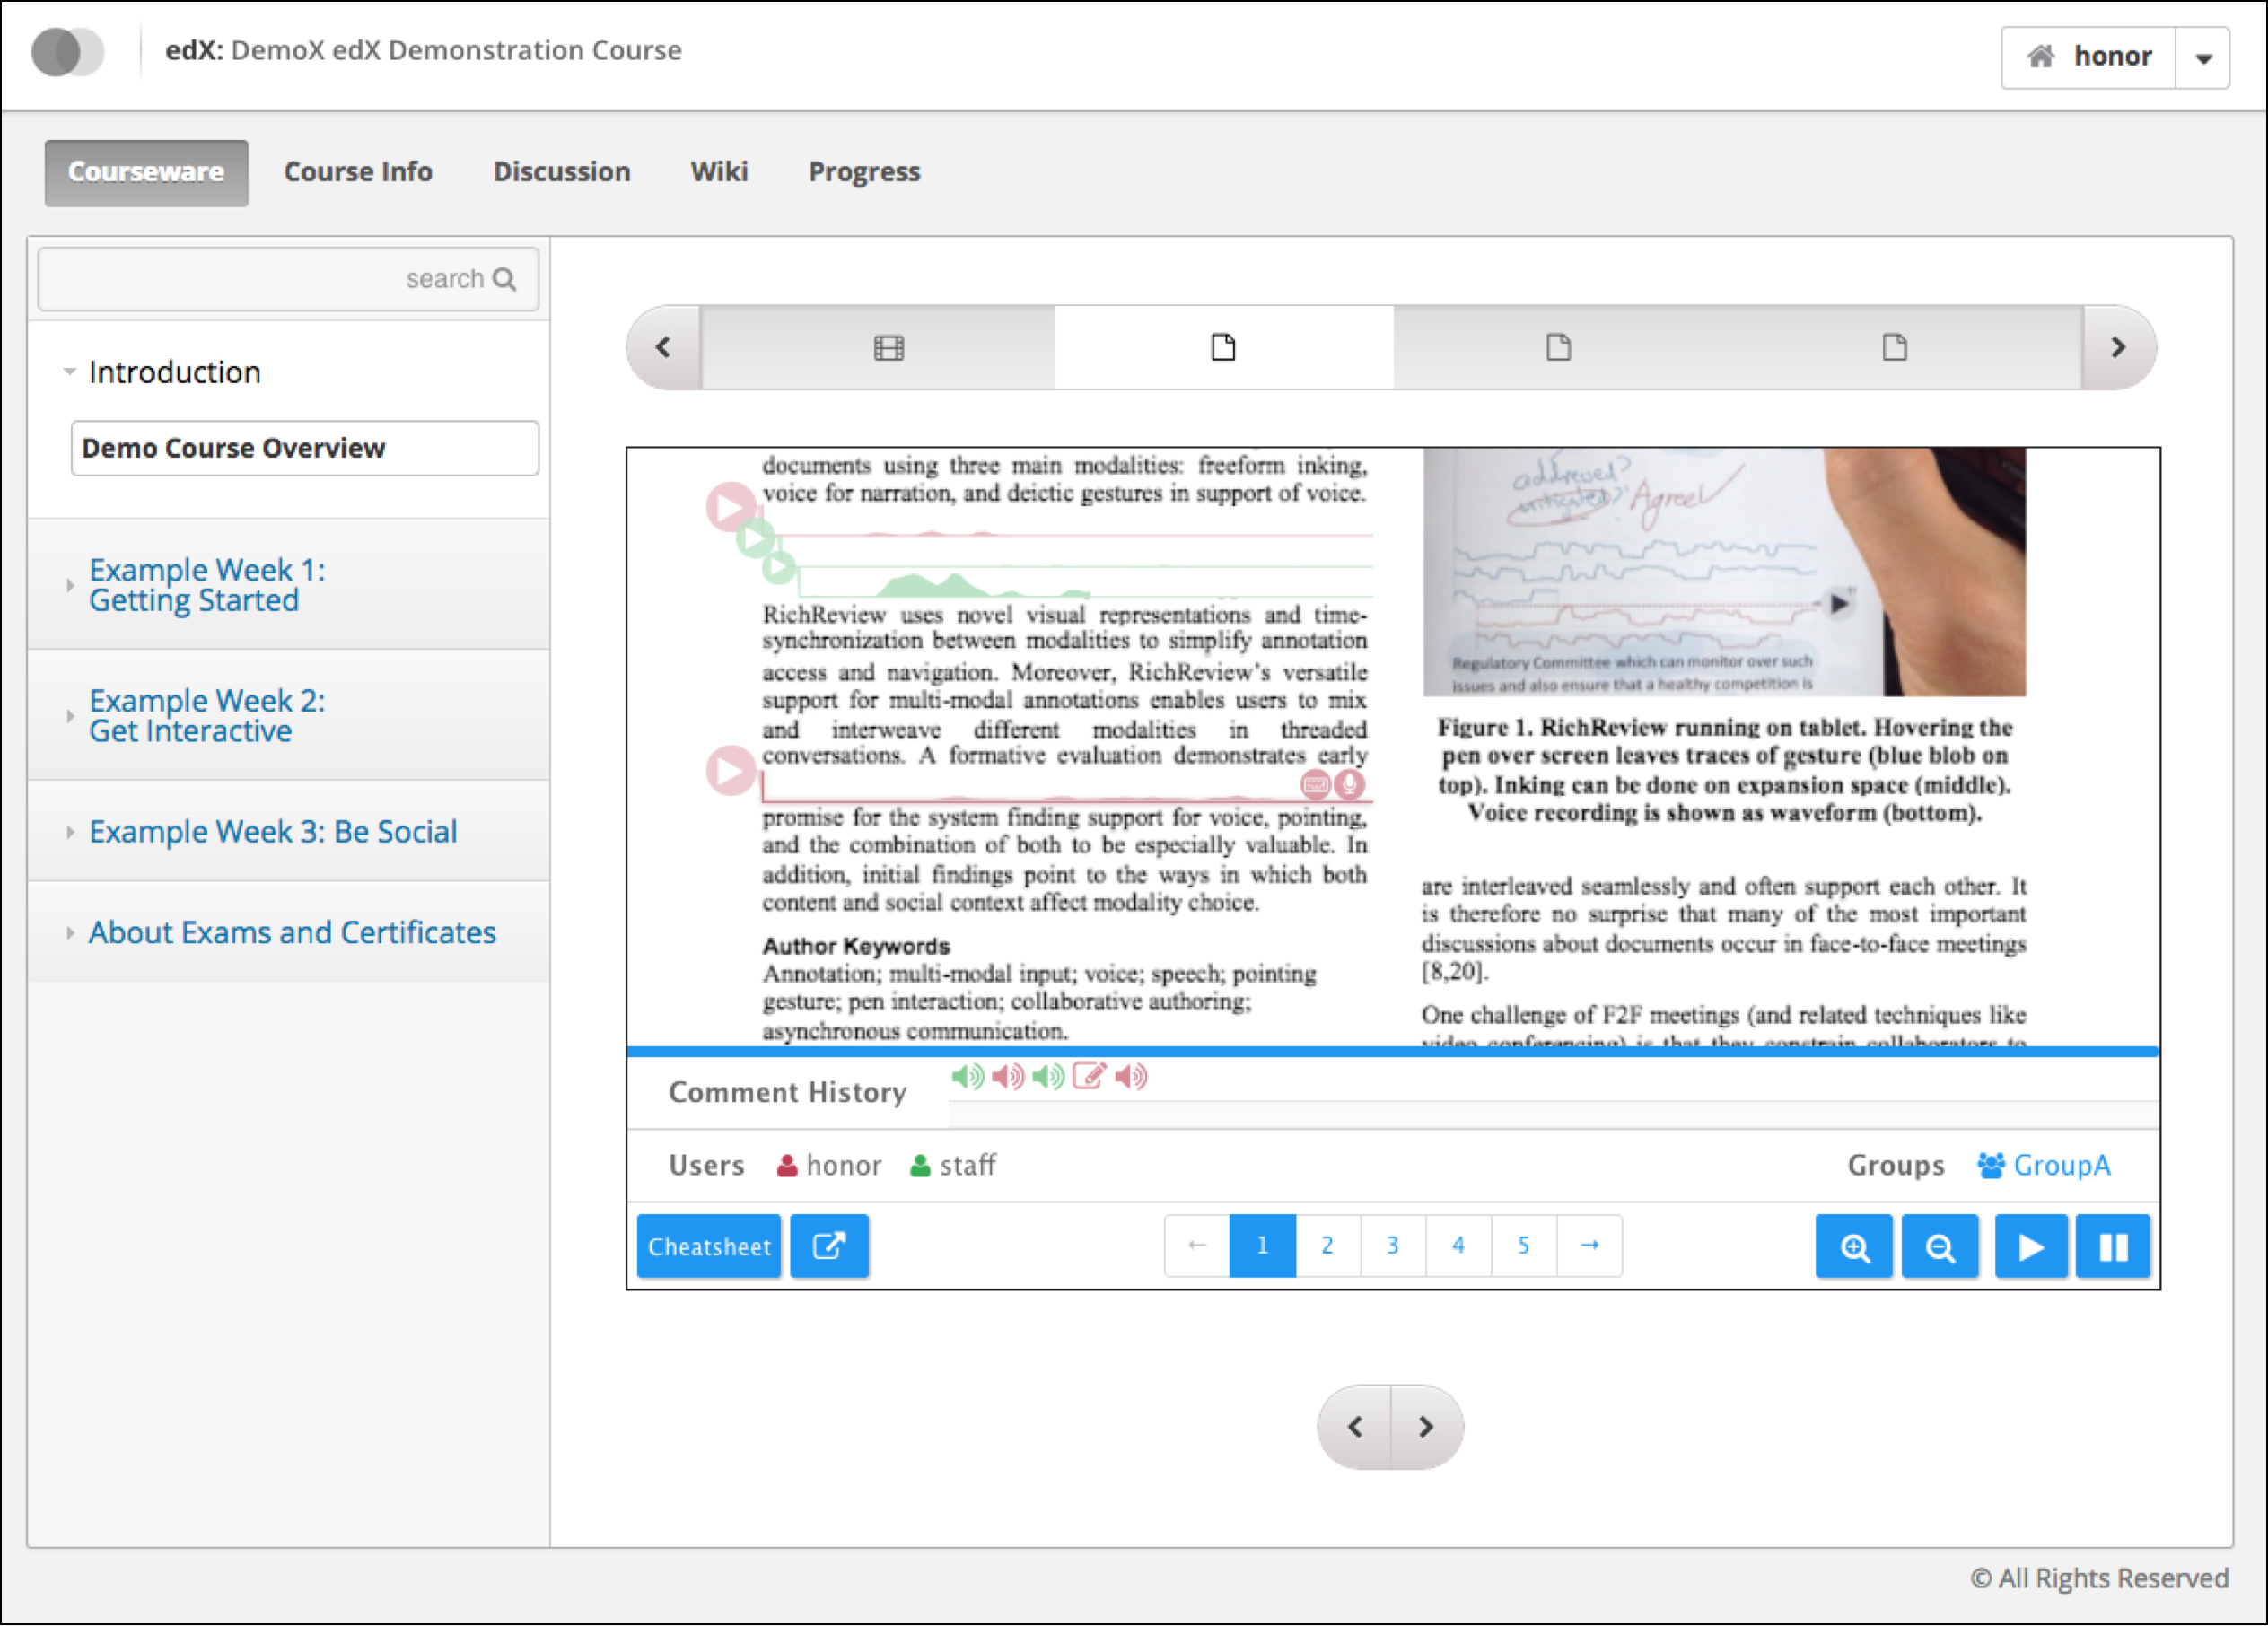
\includegraphics[width=0.95\columnwidth]{figure_edx}}
}
\caption{The RichReview web applet running in the edX courseware.}
\label{fig:figure1}
\end{figure}


\section{Previous Work: RichReview Multimodal Annotation System}
RichReview is a tablet based multimodal annotation system for bringing richness of in-person conversation into document writing revision process.
With RichReview, a commentator can record a combination of input modalities that are available in the modern tablet computers, such as digitizer writing, voice recording, and the pen's hovering.
For example, a RichReview users can verbally explain about a math concept while pointing over a relevant formula and drawing a graph.
Moreover, apart from other anchored discussion systems, RichReview puts an annotation thread within text lines of the body passage, so that the surrounding texts could enrich the context of the comments.
A prior lab study promised potential of the rich commenting system as a supporting tool for document-centric conversation.

\begin{figure}[!h]
\centering
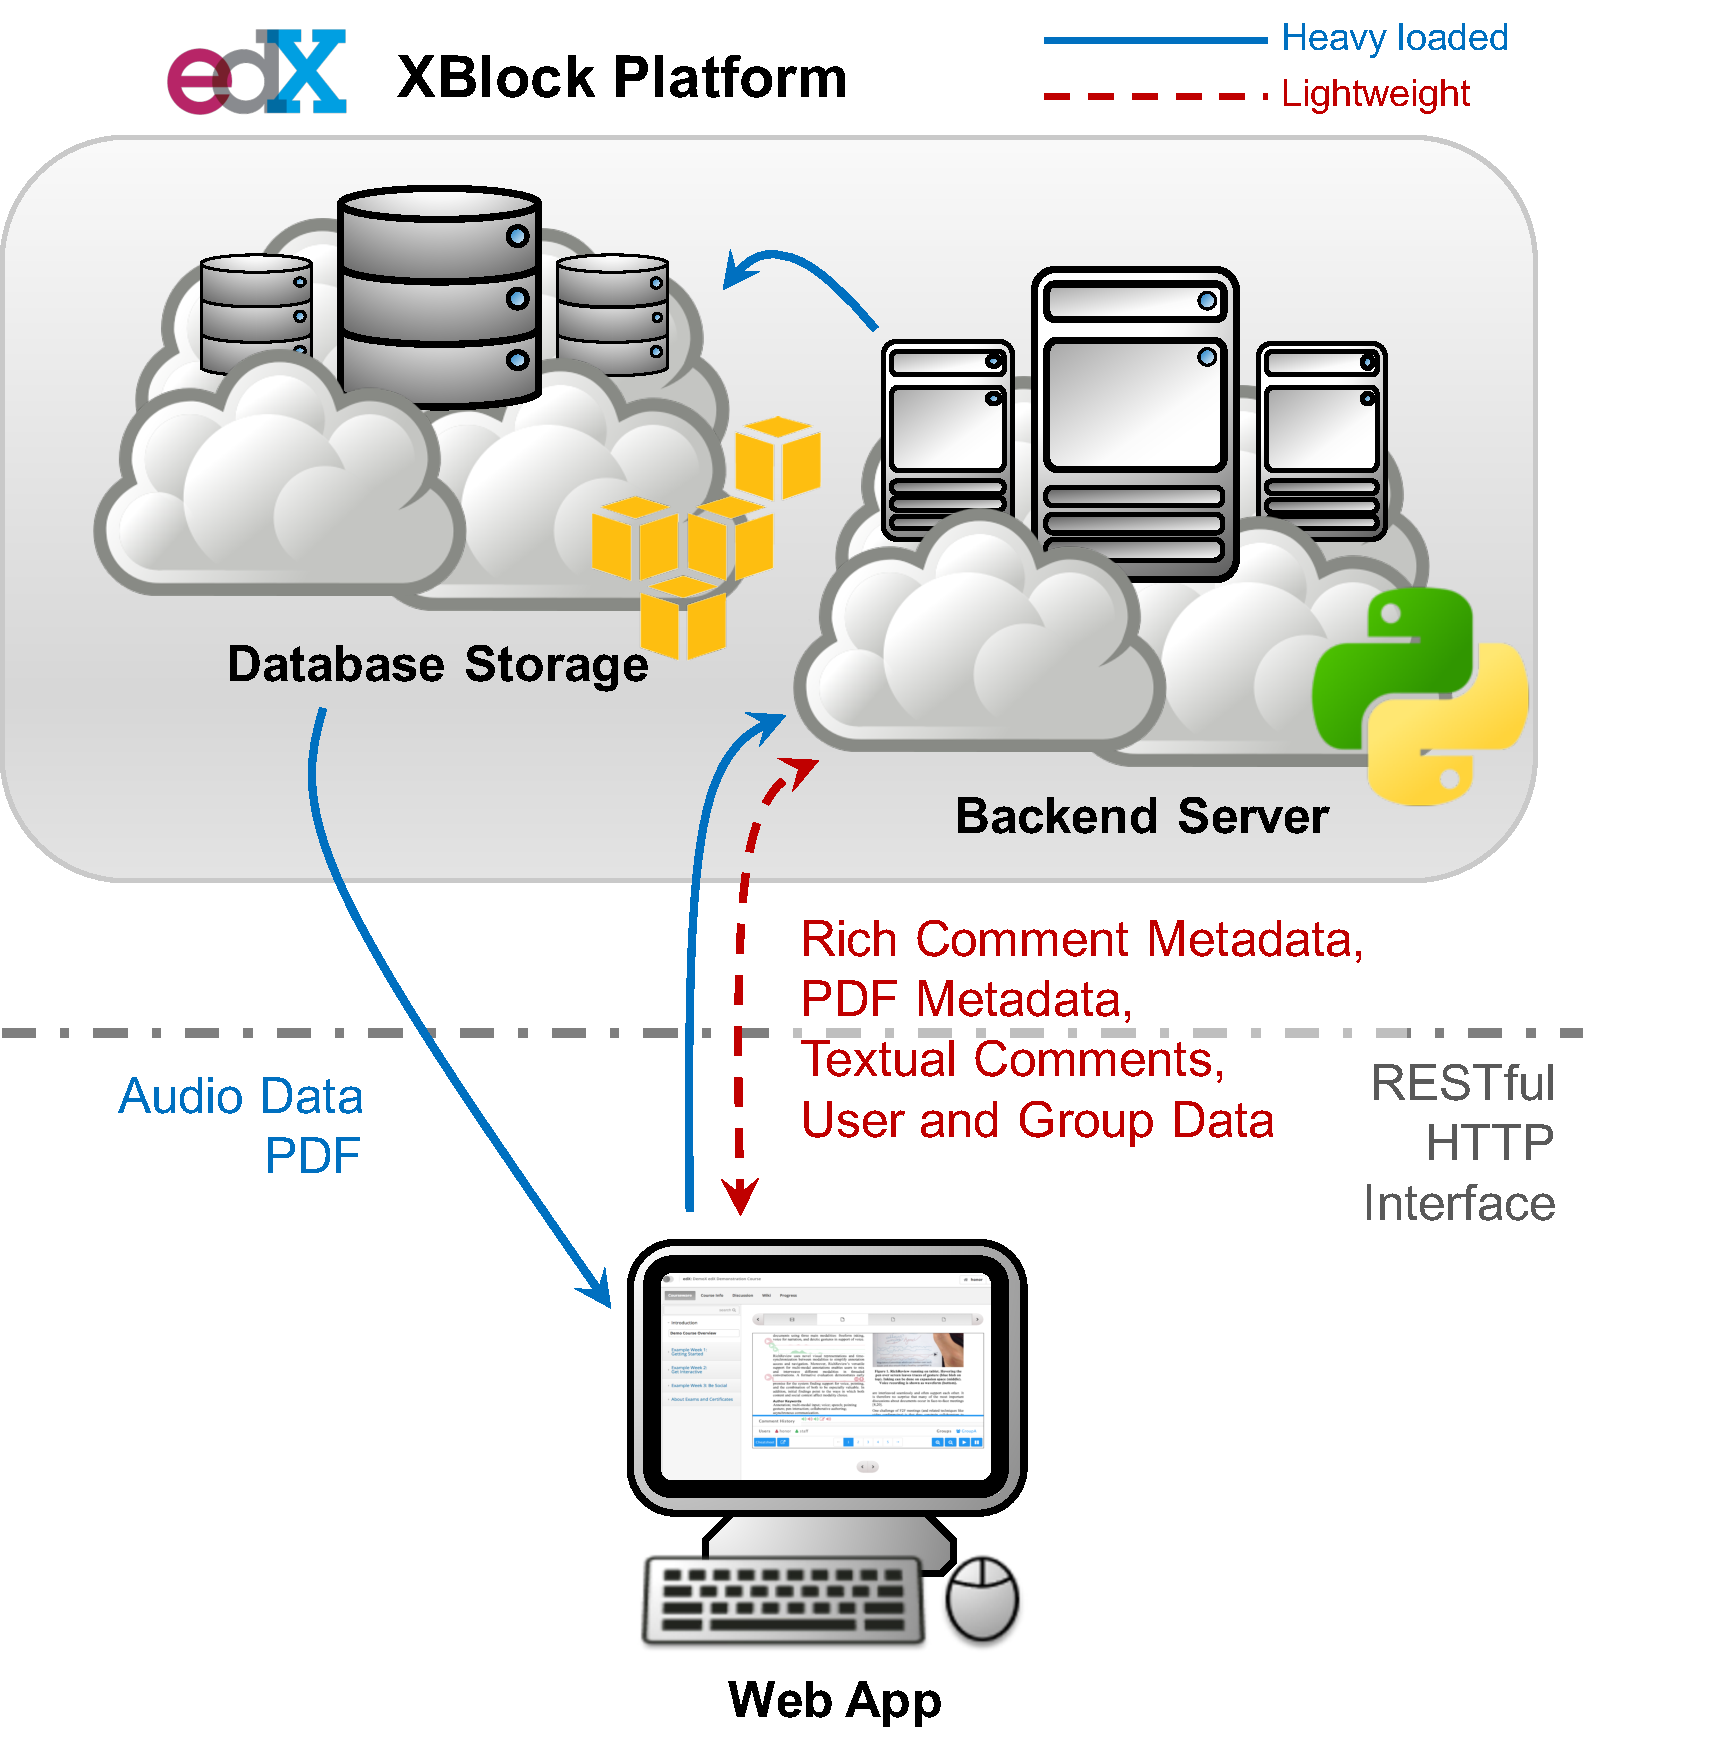
\includegraphics[width=0.95\columnwidth]{figure_architecture}
\caption{Scalable back-end architecture of the multimodal annotation system.}
\label{fig:figure2}
\end{figure}

\section{Expressive peer discussion and assessment} 

How it was implemented.

\subsection{Making the Back-end Scalable}
How I made the data flow parallel.

\subsection{Semantic Voice Editing}
Transcription based, voice editing.

\subsection{Profile Based Group-assignment}
Assigning students to groups that can maximize overall diversity of the member compositions.

\section{Acknowledgement} 
Dongwook Yoon gratefully acknowledges the support from edX and Kwanjeong educational foundation.

This format is to be used for submissions that are
published in the conference proceedings.  We wish to give
this volume a consistent, high-quality appearance. We
therefore ask that authors follow some simple
guidelines. In essence, you should format your paper
exactly like this document. The easiest way to do this is
simply to download a template from the conference web
site, and replace the content with your own material.


\bibliographystyle{acm-sigchi}
\bibliography{sample}
\end{document}
